\subsection{Problem Description} 
    The purpose of this project is to model and solve the \textit{VLSI} problem: given a fixed-width plate and a list of 
    rectangular circuits, place them on the plate so that the length of the final device is minimized. 
    
    We faced first the easier case in which the circuits cannot be rotated and then the other case on a distinct model.

    The solution of the problem gives the position of each circuit (the coordinates of the bottom left corner) and,
    in case a circuit has been rotated, its width and height are coherently modified.
    \colorbox{BurntOrange}{TODO improve ...}

% % % % % % % % % % % % % % % % % % % % % % % % % % % % % % % % % % % % % % % % % % % % % % % % % %

\subsection{Format of the Instances}
    \paragraph*{Instance Format}
        An instance of \textit{VLSI} is a text file consisting of lines of integer values. The first line gives \textit{width}, 
        which is the width of the silicon plate. The following line gives \textit{nc}, which is the number of necessary circuits 
        to place inside the plate. Then \textit{nc} lines follow, each with $w_i$ and $h_i$, representing the horizontal and 
        vertical dimension of the \textit{i-th} circuit.

    \paragraph*{Solution Format}
        A solution of \textit{VLSI} is a text file built starting from the input file. To the first line is added the \textit{makespan},
        which is the length of the final device. The second line is kept the same while to the following \textit{nc} lines are added
        $x_i$ and $y_i$, which are the coordinates of the bottom left corner of the \textit{i-th} circuit. In case a solution is obtained 
        through the rotation of a circuit $i$, then, in the output file, the horizontal and vertical dimensions ($w_i$ and $h_i$) 
        will be swapped w.r.t. the input text file.

    \colorbox{BurntOrange}{TODO improve ...}

% % % % % % % % % % % % % % % % % % % % % % % % % % % % % % % % % % % % % % % % % % % % % % % % % %

\subsection{Shared Variables Declaration}
    In this section we list the constants and the variables that are shared in the mathematical formalization of 
    models and constraints from now on.

    Constant values:
    \begin{align*}
        nc\             &\ =\ \text{total number of circuits}                   \\
        width\          &\ =\ \text{width of the plate}                         \\
        c_i\            &\ =\ \text{index of circuit  } i                       \\
        w_i\            &\ =\ \text{width of circuit  } i                       \\
        h_i\            &\ =\ \text{height of circuit  } i                      \\
        min\_makesapan  &\ =\ \text{lower bound of \textit{makespan} variable}  \\
        max\_makesapan  &\ =\ \text{upper bound of \textit{makespan} variable}  \\
        % C\              &\ =\ \bigcup_{i=1}^{nc} c_i                            \\
        C\              &\ =\ \{ c_i\ |\ i \in [1, nc]\}                         \\        
        CC\             &\ =\ \{(i, j) \in C \times C\ |\ i<j \}
    \end{align*}

    Variables:
    \begin{align*}
        x_i\        &\ =\ \text{x coordinate of the bottom-left corner of circuit  } i        \\
        y_i\        &\ =\ \text{y coordinate of the bottom-left corner of circuit  } i        \\
        r_i\        &\ =\ \text{boolean variable indicating if circuit \textit{i} is rotated} \\
        % X\          &\ =\ \bigcup_{c=1}^{nc} x_c                                              \\
        % Y\          &\ =\ \bigcup_{c=1}^{nc} y_c                                              \\
        X\          &\ =\ \{ x_i\ |\ i \in [1, nc]\}                                          \\
        Y\          &\ =\ \{ y_i\ |\ i \in [1, nc]\}                                          \\
        Xcross(x)\  &\ =\ \{ c \in C\ |\ (x_c \leq x) \land (x_c + w_c > x) \}                \\
        Ycross(y)\  &\ =\ \{ c \in C\ |\ (y_c \leq y) \land (y_c + h_c > y) \}                \\
        makespan\   &\ =\ \max_{c \in C}\ y_c + h_c
    \end{align*}
    \colorbox{BurntOrange}{TODO: uniformare pedici}

    \subsubsection{Makespan lower bound}
        In order to limit the search domain of the \textit{makespan} variable, we defined an algorithm to find 
        its lower (\textit{min\_makespan}) and upper (\textit{max\_makespan}) bound.

        The lower bound is determined starting from the area that the circuits occupy: 
        \begin{equation}
            a = \sum_{c \in C} w_c \cdot h_c
        \end{equation}
        The best situation is the one in which all circuits fit in the plate 
        without leaving any empty space, so that the \textit{makespan} would be $makespan = \lceil a / width \rceil$. 
        We could set accordingly $min\_makespan = \lceil a / width \rceil$, but there is a case in which,
        even if there are no empty spaces left, the \textit{makespan} is not the one defined before. 
        Indeed, we may have a very "high" circuit (let's name it $c_{high}$) such that:
        \begin{equation}
            h_{c_{high}} >= \lceil \frac{\sum_{c \in C - \{c_{high}\}} w_c \cdot h_c}{width - w_{c_{high}}} \rceil
            \label{eq:h_high}
        \end{equation}
        where the numerator is the sum of the areas of all circuits $c_i \neq c_{high}$, obtaining on the right of
        the inequality the $min\_makespan'$ without $c_{high}$ and with $width' = width - w_{c_{high}}$.

        Let's call $m$ the right side of the inequality, it's almost intuitive that the $min\_makespan$ computed
        as before is lower than $h_{c_{high}}$:
        \begin{equation}
            m\ =\ \frac{\sum_{c \in C - \{c_{high}\}} w_c \cdot h_c}{width - w_{c_{high}}}
            \label{eq:m}
        \end{equation}
        then
        \begin{align*}
            min\_makespan\  &\ =\ m + \frac{(h_{c_{high}} - m) \cdot w_{c_{high}}}{width}                                               \\
                            &\ =\ h_{c_{high}} \cdot \frac{w_{c_{high}}}{width} + m \cdot \left(1 - \frac{w_{c_{high}}}{width}\right)   \\
            h_{c_{high}}\   &\ =\ \frac{width}{w_{c_{high}}} \cdot min\_makespan - \left( \frac{width}{w_{c_{high}}} - 1\right) \cdot m
        \end{align*}

        From the first one we have $min\_makespan \geq m$ since $h_{c_{high}} \geq m$ for definition.
        From the second we can easily proof $h_{c_{high}} \geq min\_makespan$:
        \begin{align*}
            h_{c_{high}}\ =\ \frac{width}{w_{c_{high}}} \cdot min\_makespan - \left( \frac{width}{w_{c_{high}}} - 1\right) \cdot m\ &\ \geq\ min\_makespan       \\
            \left( \frac{width}{w_{c_{high}}} - 1\right) \cdot min\_makespan - \left( \frac{width}{w_{c_{high}}} - 1\right) \cdot m\ &\ \geq\ 0 \\
            \left( \frac{width}{w_{c_{high}}} - 1\right) \cdot \left(min\_makespan - m\right) \ &\ \geq\ 0
        \end{align*}
        that is true since $width \geq w_{c_{high}} \rightarrow \frac{width}{w_{c_{high}}} \geq 1$ and $min\_makespan \geq m$ as shown before;
        the situation we are describing is also shown in Fig.\ref{fig:min_makespan}. 

        \begin{figure}[H]
            \centering
            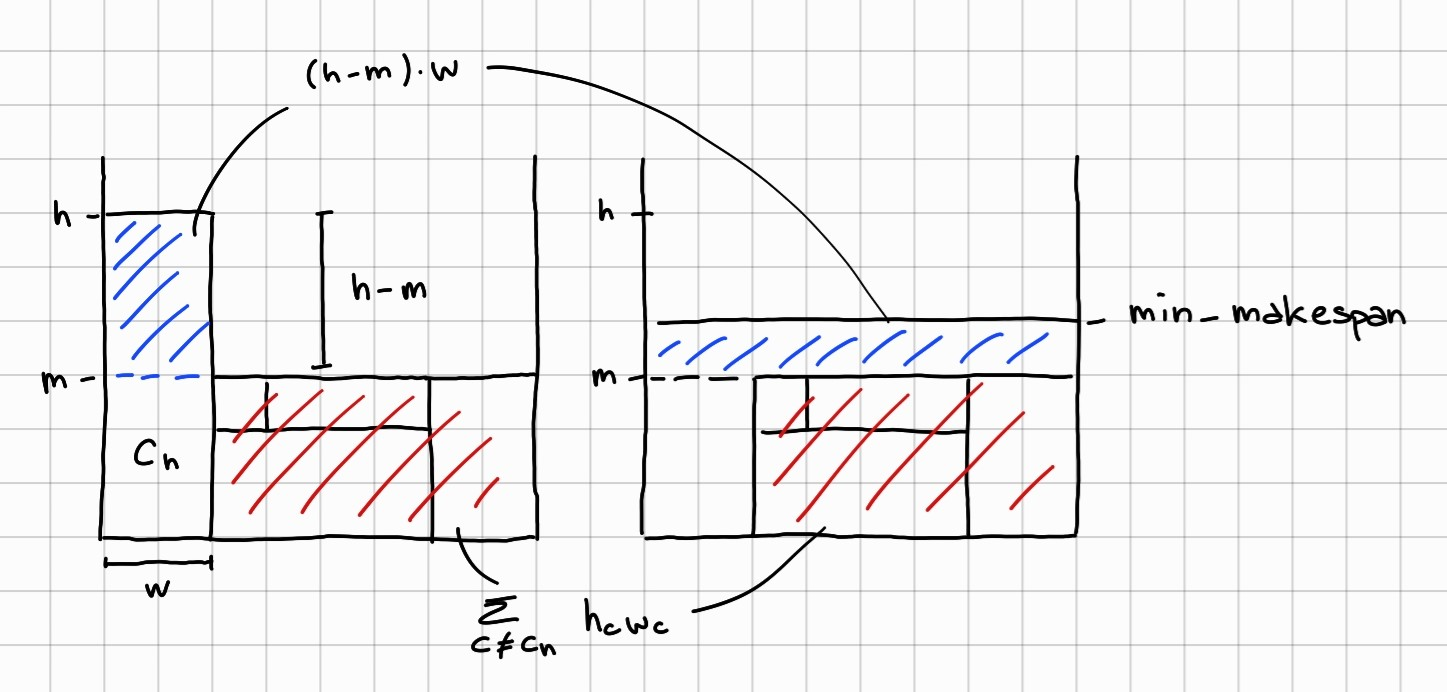
\includegraphics[width=0.6\textwidth]{min_makespan_exc.jpg}
            \caption{
                On the left a possible solution with circuit $c_n=c_{high}$ satisfying condition \ref{eq:h_high}, 
                with $m$ defined in \ref{eq:m} and $h = h_{c_{high}}$. On the right, how $min\_makespan$ was taken before
                improving it. In this situations we always have $m \leq min\_makespan \leq h_{c_{high}}$.
            }
            \label{fig:min_makespan}
        \end{figure}
        
        The improvement for the lower bound of $makespan$ is easy and immediate:
        \begin{equation}
            min\_makespan\ =\ max\left(\max_{c \in C} h_c, \lceil a / width \rceil\right)
        \end{equation}

    \subsubsection{Makespan upper bound}
        The upper bound of the \textit{makespan} variable (\textit{max\_makespan}) is determined as the makespan of a possible 
        solution. The solution must be built using an effective and efficient algorithm. 
        The solution with the greatest possible \textit{max\_makespan} is obtained stacking one on top of the other all the circuits
        of the instance. This strategy is very simple and fast but the result easily over estimates by a lot the final 
        \textit{makespan} value. A more effective strategy was adopted.
        
        A much better algorithm requires to consider each circuit as a node and to build a possible solution building a tree of the nodes. 
        Each circuit is represented as a node that contains the dimensions of the circuit $w_c$, $h_c$, its coordinates 
        $x_c$, $y_c$, the index of the circuit, the index of the parent node and a list of the children nodes 
        $children\_list$. The $altitude$ of the node can be computed as:
        \begin{equation}
            altitude_c = y_c + h_c
        \end{equation}
        The remaining horizontal free space \textit{remaining\_space} on the top of each circuit can be calculated as:
        \begin{equation}
            remaining\_space_c = w_c - \sum_{i \in children\_list} w_i
        \end{equation}
        
        The relationship of a circuit being stacked on top of another is represented with the node of the circuit at the bottom 
        being the father of the node of the circuit stacked on top.
        A conceptual root node is computed. The width of the root node is the $width$ of the plate and its height is 0.
        All the other nodes are added to a list of nodes.
        First the list of nodes is sorted on the width of the circuit in descending order:
        \begin{equation}
            w_i \geq w_j \Longleftrightarrow i \leq j\   \ \forall (i,j) \in CC
        \end{equation}
        \colorbox{BurntOrange}{abbiamo già $i < j$ per definizione di CC, secondo me basta $w_i \geq w_j \ \forall (i,j) \in CC$}

        In this way the nodes are added to the tree from the widest to the least wide.
        The nodes are then inserted into the tree using the following strategy. A list of possible parent nodes $fringe$ is kept. 
        A node to be a parent of another must have enough free space on top. Let $x$ be the circuit that 
        is being inserted. $fringe$ is the list of all the nodes $c$ already in the tree that satisfy: 
        \begin{equation}
            w_x \leq w_c - \sum_{i \in children\_list_c} w_i
        \end{equation}
        
        Each new node is appended to the node in the fringe whose altitude is the lowest.
        \begin{equation}
            altitude_{father} = \min_{c \in fringe}\ {altitude_c} 
        \end{equation}

        Once all the nodes are in the tree we can calculate the maximum altitude $altitude_{max}$ reached by the nodes.
        \begin{equation}
            altitude_{max} = \max_{c \in C}\  altitude_c
        \end{equation}

        This value is the makespan of a fully legit solution so it is intuitive that the makespan of the best solution cannot
        be greater than it. 
        
        The time required for this calculation is negligible w.r.t the time required to obtain the best solutions with any 
        of the technologies used.

    \subsubsection{Rotation}
        \colorbox{BurntOrange}{TODO missing ... se dobbiamo metterci solo $r_i$ forse questa sezione non serve ...}



\subsection{Shared Constraints Declaration}
    The following formalization will be the one followed for the CP solution and then adapted for SAT and SMT. 
    The LP model will be described later.

    \begin{align*}
           w_c > 0\ \ \land\ &\ w_c \leq width\    &\ \hspace{0.2cm} \forall c \in C \\
           h_c > 0\ \ \land\ &\ h_c \leq makespan\ &\ \hspace{0.2cm} \forall c \in C \\
        x_c \geq 0\ \ \land\ &\ x_c < width\    &\ \hspace{0.2cm} \forall c \in C \\
        y_c \geq 0\ \ \land\ &\ y_c < makespan\ &\ \hspace{0.2cm} \forall c \in C
    \end{align*}

    \begin{align}
        (x_i + w_i \leq x_j) \lor (y_i + h_i \leq y_j) &\ \ &\ \nonumber \\
        \lor\ (x_j + w_j \leq x_i) \lor (y_j + h_j \leq y_i)\ &\                \hspace{0.2cm} \forall (i,j) \in CC &\ \text{;diffn} \\
        \sum_{c \in C_x} y_c \leq makespan\ &\ \hspace{0.2cm} \forall x \in X, \forall c \in Xcross(x)\ &\ \text{;x axis} \\
        \sum_{c \in C_y} x_c \leq width\ &\ \hspace{0.2cm} \forall y \in Y, \forall c \in Ycross(y)\ &\ \text{;y axis}
    \end{align}

    \subsubsection{Symmetries}
    \colorbox{BurntOrange}{TODO controllare assolutamente formulazione delle frasi ...}


        Given a solution there are two main ways to get a different one with the same \textit{makespan}:
        swap circuits with same dimensions [Fig.\ref{fig:symmetry_swap}] or get the solution specular w.r.t. the horizontal 
        or vertical axis [Fig.\ref{fig:symmetry_specular}].
        If we consider also sub-rectangles which do not cross their edges with any circuit and call them 
        \textit{virtual} circuits [Fig.\ref{fig:virtual circuit}], we can generalize what mentioned before and find all solutions with 
        the same \textit{makespan} [Fig.\ref{fig:symmetry_vc}].
        In particular we can find a symmetric solution swapping any couple of circuits or \textit{virtual} circuits 
        with same dimensions. Another possibility is to substitute any \textit{virtual} circuit with the set of regular circuits within it, 
        but with specular positions. Obviously, any combination of the previous cases will create other symmetric 
        solutions [Fig.\ref{fig:vc_specular_out}].

        \begin{figure}[H]
            \centering
            \begin{subfigure}[b]{0.45\textwidth}
                \centering 
                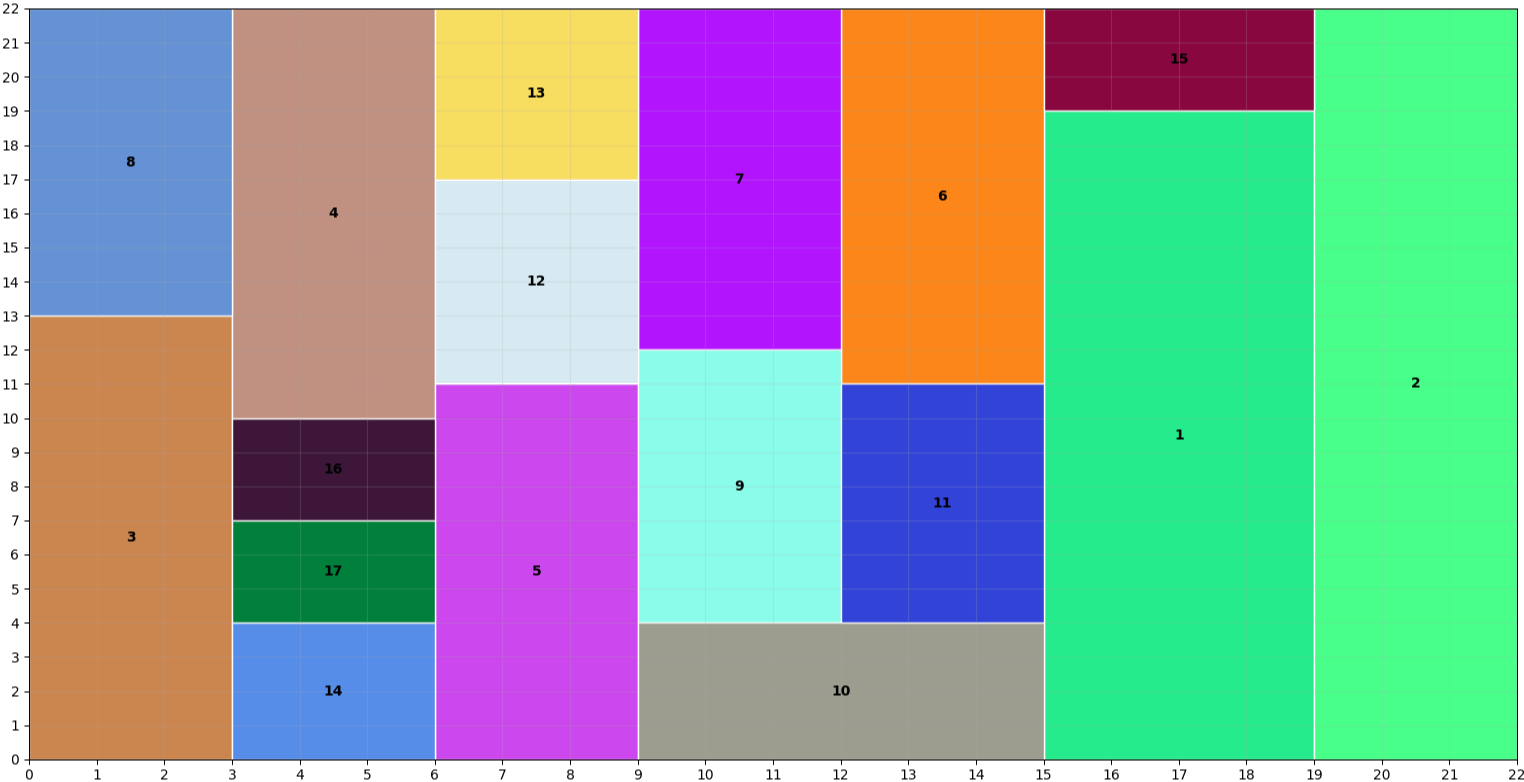
\includegraphics[width=\textwidth]{ins_15.png}
                \caption{}
                \label{fig:ins_15_mod}
            \end{subfigure}
            \hfill
            \begin{subfigure}[b]{0.45\textwidth}
                \centering
                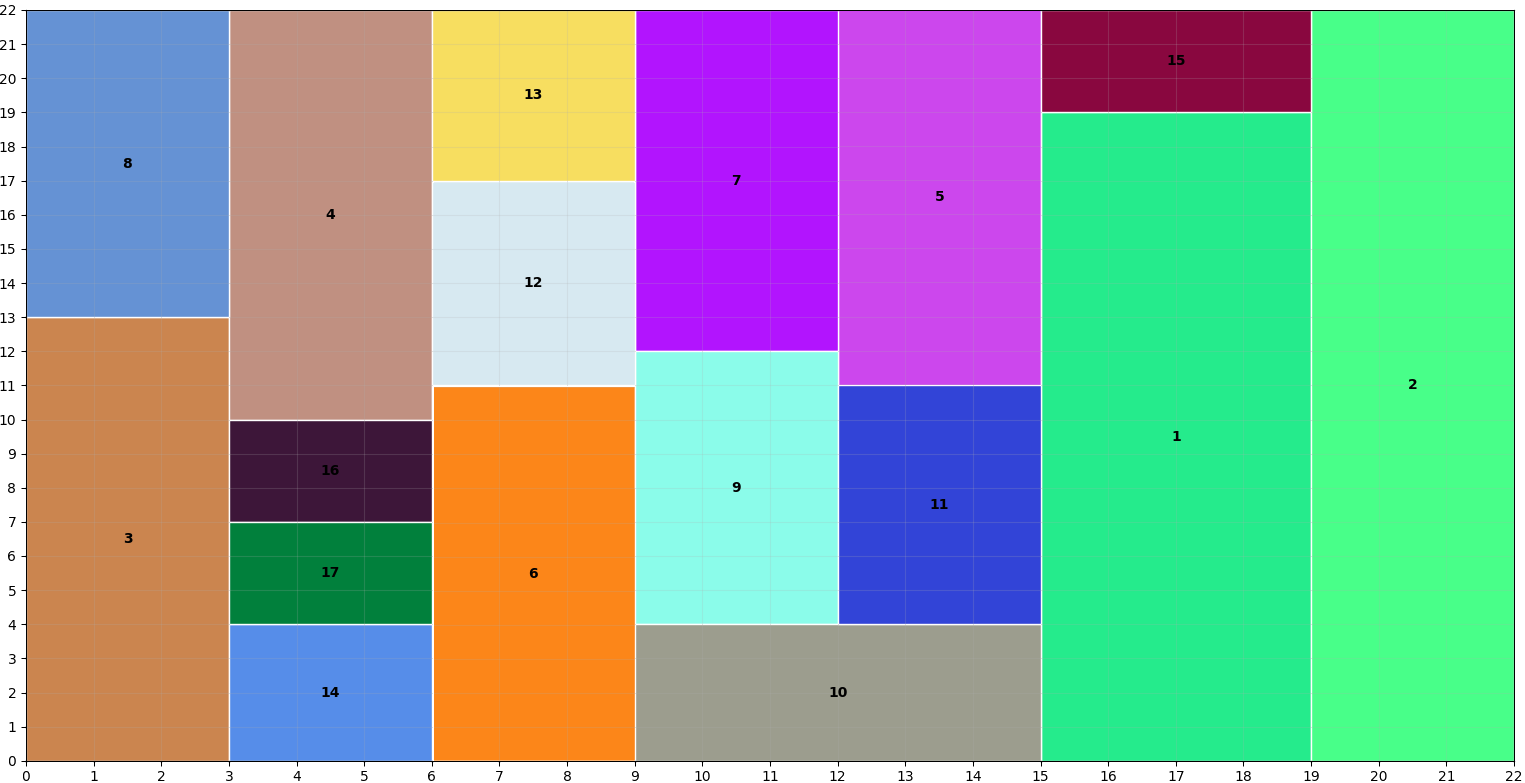
\includegraphics[width=\textwidth]{ins_15_swap.png}
                \caption{}
                \label{fig:ins_15_swap}
            \end{subfigure}
            \hfill
            \caption{
                Plotted solution of an instance created for explanatory puropose.
                From the solution on the left \ref{fig:ins_15_mod} we can create a different one
                with the same \textit{makespan} just swapping circuits with same dimensions. In
                the plot on the right \ref{fig:ins_15_swap} we swapped circuit 5 (at originial
                position of (6,0)) and circuit 6 (at originial position of (12,11)).
            }
            \label{fig:symmetry_swap}
        \end{figure}
       
        \begin{figure}[H]
            \centering
            \begin{subfigure}[b]{0.45\textwidth}
                \centering
                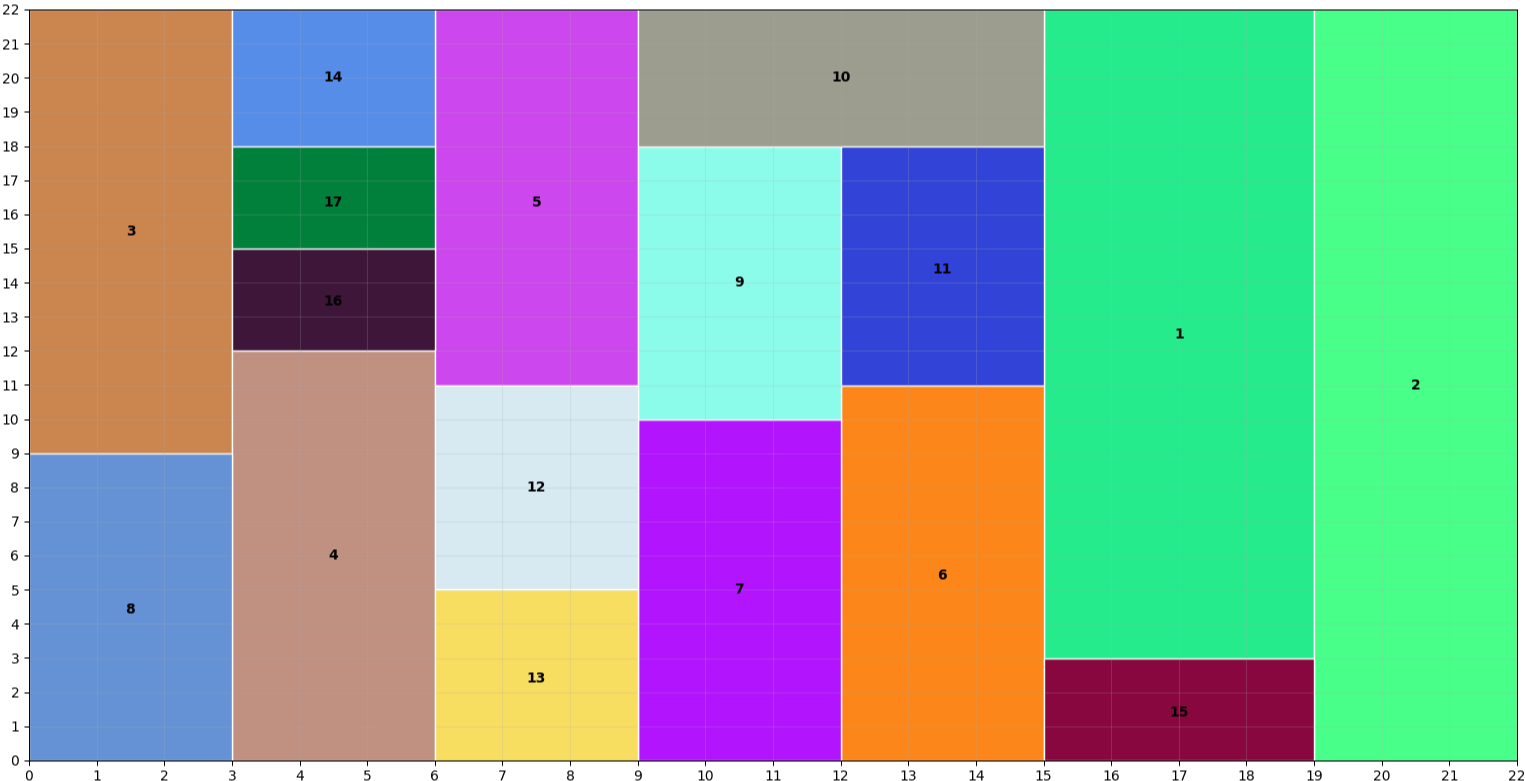
\includegraphics[width=\textwidth]{ins_15_specular_v.png}
                \caption{}
                \label{fig:ins_15_specular_v}
            \end{subfigure}
            \hfill
            \begin{subfigure}[b]{0.45\textwidth}
                \centering 
                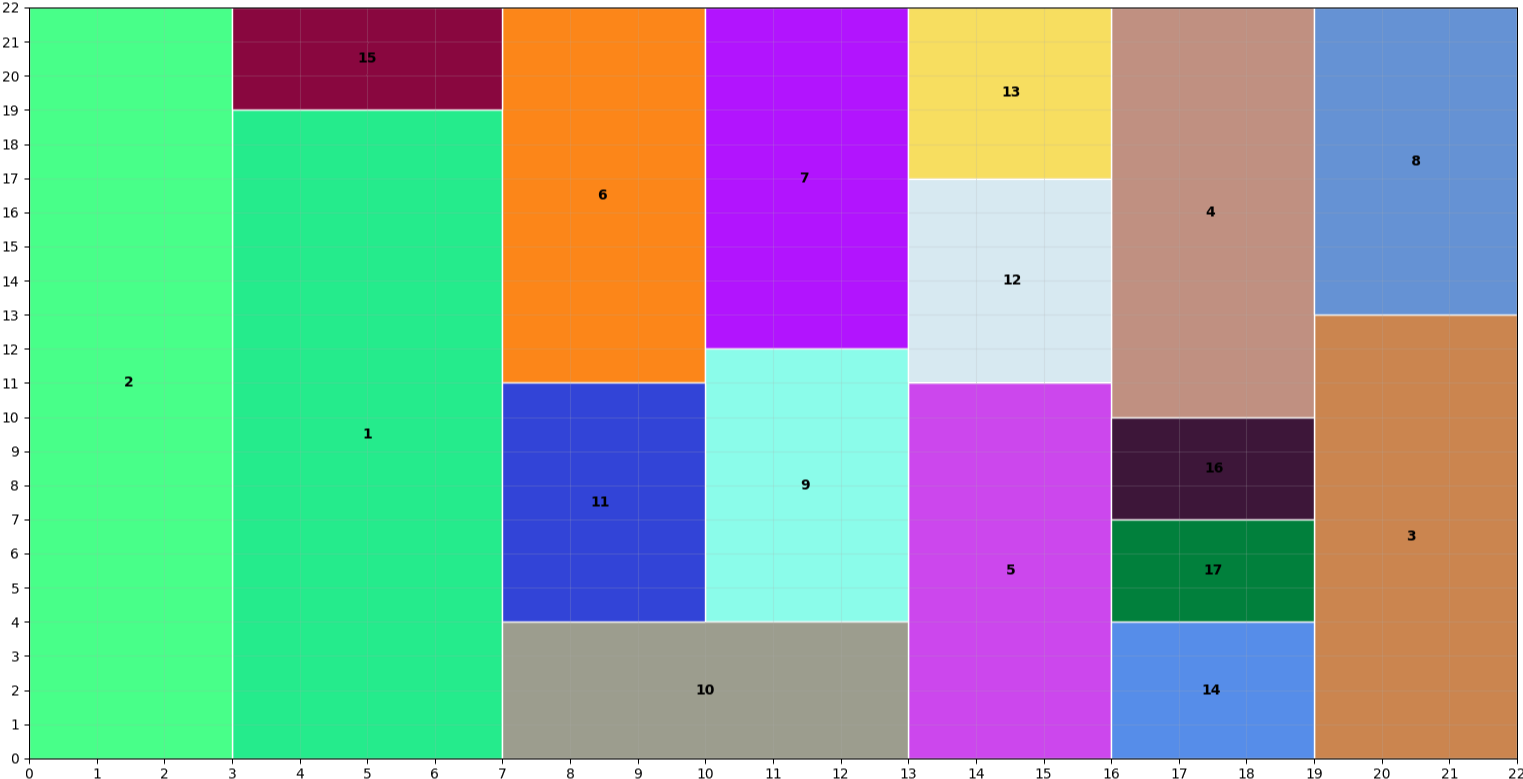
\includegraphics[width=\textwidth]{ins_15_specular_h.png}
                \caption{}
                \label{fig:ins_15_specular_h}
            \end{subfigure}
            \hfill
            \caption{
                Other possible solutions with same makespan as the one plotted in \ref{fig:ins_15_mod}.
                The left one \ref{fig:ins_15_specular_h} is the specular w.r.t. the vertical axis,
                while the left one \ref{fig:ins_15_specular_v} is the specular w.r.t. the horizontal axis
            }
            \label{fig:symmetry_specular}
        \end{figure}

        \begin{figure}[H]
            \centering
            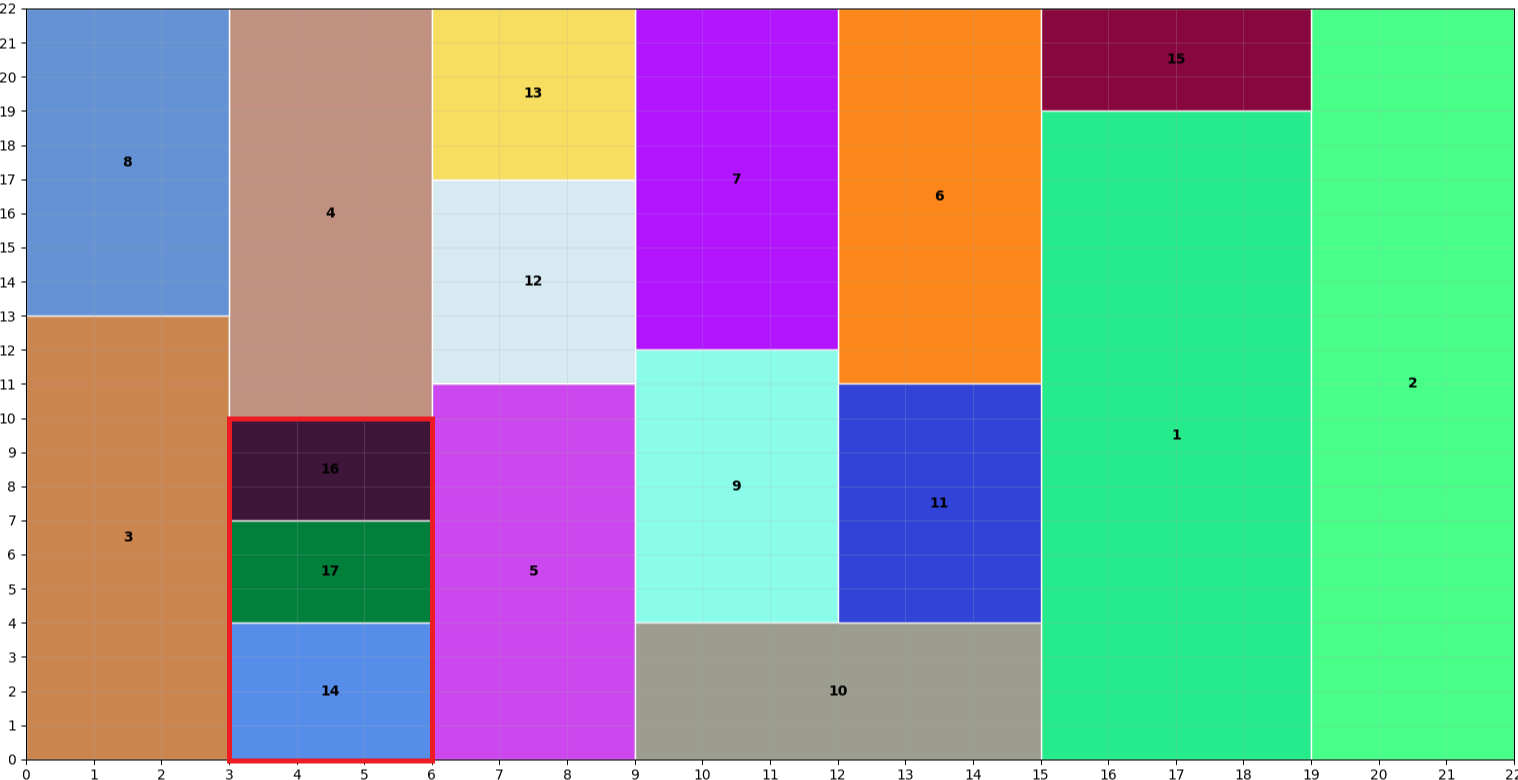
\includegraphics[width=0.5\textwidth]{ins_15_vc.png}
            \caption{
                At position $(3,0)$ an example of \textit{virtual} circuit highlighted in red,
                with $w = 3$ and $h = 10$, which includes inside the circuits 14, 16 and 17.
            }
            \label{fig:virtual circuit}
        \end{figure}

        \begin{figure}[H]
            \centering
            \begin{subfigure}[b]{0.3\textwidth}
                \centering 
                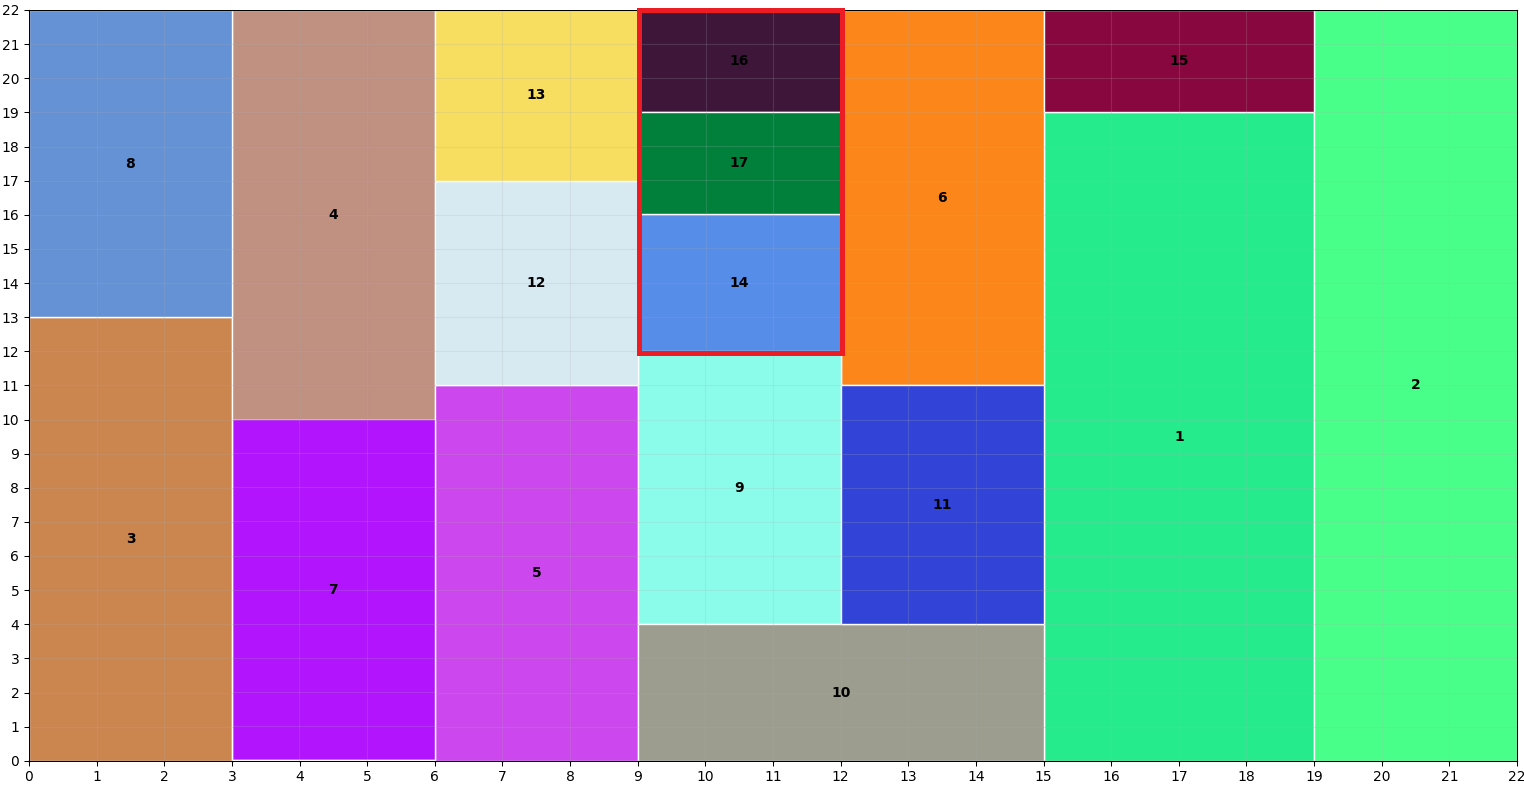
\includegraphics[width=\textwidth]{ins_15_vc_swap.png}
                \caption{}
                \label{fig:vc_swap}
            \end{subfigure}
            \hfill
            \begin{subfigure}[b]{0.3\textwidth}
                \centering
                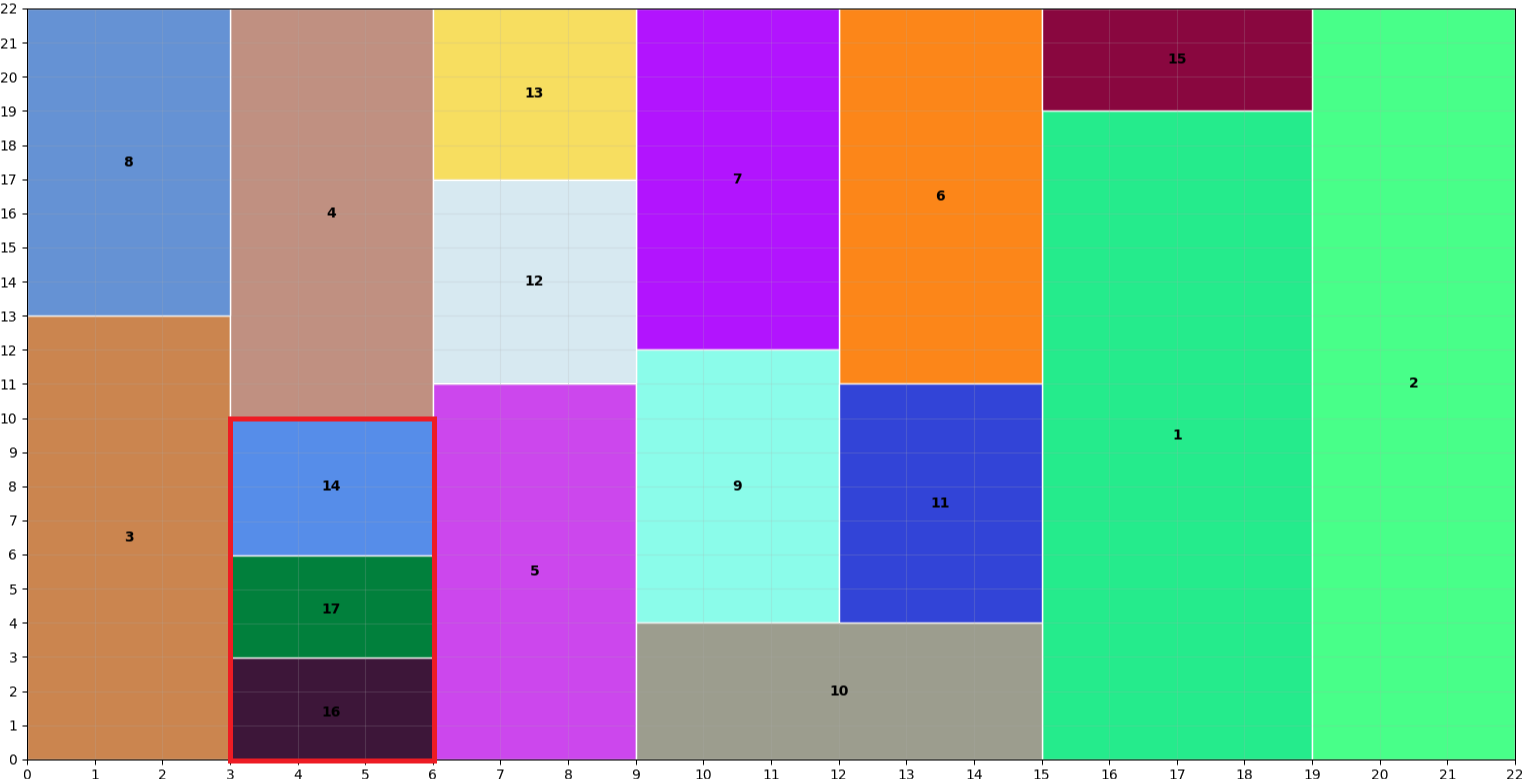
\includegraphics[width=\textwidth]{ins_15_vc_specular_in.png}
                \caption{}
                \label{fig:vc_specular_in}
            \end{subfigure}
            \hfill
            \begin{subfigure}[b]{0.3\textwidth}
                \centering
                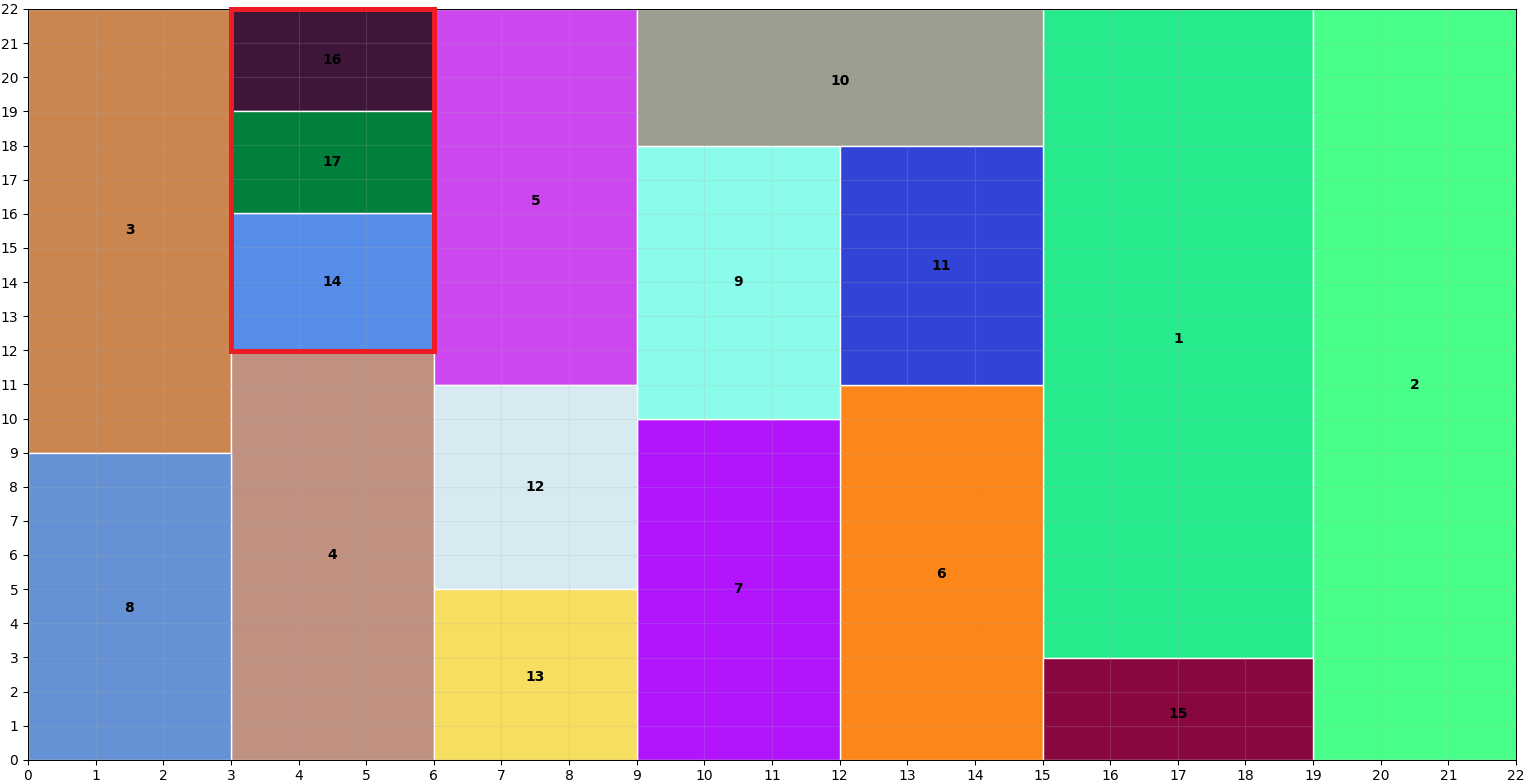
\includegraphics[width=\textwidth]{ins_15_vc_specular_out.png}
                \caption{}
                \label{fig:vc_specular_out}
            \end{subfigure}
            \caption{
                Other possible solutions with same makespan as the one plotted in \ref{fig:ins_15_mod},
                now including also \textit{virtual} circuits in the reasoning.
                In the left one \ref{fig:vc_swap}, the \textit{virtual} circuit introduced in Fig.\ref{fig:virtual circuit}
                at original position (3,0) is swapped with the regular circuit 7 at original position (9,11).
                In the middle one \ref{fig:vc_specular_in} the same \textit{virtual} circuit is substituted with 
                its specular w.r.t. the horizontal axis.
                The right one \ref{fig:vc_specular_out} is an example of combination of what mentioned before:
                starting from the solution \ref{fig:ins_15_specular_v}, the subset of circuits 14, 16, 17, belonging to 
                the highlighted \textit{virtual} circuit, is \textit{"mirrored"} again.
            }
            \label{fig:symmetry_vc}
        \end{figure}

        Catching all the symmetric solutions described before is quite demanding and we did not find an 
        efficient way of implementing symmetry breaking constraints, so we tried to keep them as simple 
        as possible.

        Let's define first some support variables:
        \begin{align*}
            x\_v\   &\ =\ [x_c\ |\ c \in C]                     \\
            y\_v\   &\ =\ [y_c\ |\ c \in C]                     \\
            x\_v'\  &\ =\ [width - (x_c + w_c)\ |\ c \in C]     \\
            y\_v'\  &\ =\ [makesapan - (y_c + h_c)\ |\ c \in C] \\ 
            \label{eq:specular_coord}
        \end{align*}
        where $x\_v$ and $y\_v$ are respectively the vector of all horizontal and vertical coordinates,
        while $x\_v'$ and $y\_v'$ are the horizontal and the vertical coordinates of the specular circuits.

        The symmetry breaking constraints proposed for CP, SAT and SMT are the lexicographic orderings
        between $y\_v$ and $y\_v'$ and between $x\_v$ and $x\_v'$; in this way we break the 
        symmetries shown respectively in Fig.\ref{fig:ins_15_specular_v} and Fig.\ref{fig:ins_15_specular_h}.

        Anyway, later we will specify better the adopted constraints and compare the performances of the 
        CP, SAT and SMT models with and without the symmetry breaking constraints.
